 \documentclass[book.tex]{subfiles}
\begin{document}

\section{Tricks}

This section describes random tricks used to speed up rendering. 




\subsection{Bouncing Flower Lookup}
When Keen throws a flower it bounces of the walls. For flat walls and floors the bounce can be easily calculated by reversing either the x-speed (for vertical walls) or y-speed (for horizontal walls). It becomes more complicated for slopes. Making an accurate calculation of the bounce on a slope requires expensive \cw{cos} and \cw{sin} methods. This involves floating point calculations, which are expensive to use. \\
\par
Instead, the game used a simple algorithm that approximates the angle to either 22$^{\circ}$, 45$^{\circ}$ or 90$^{\circ}$. Based on the ratio between the x- and y-speed it calculates the resulting speed and corresponding angle.\\
\par
\begin{figure}[H]
\centering
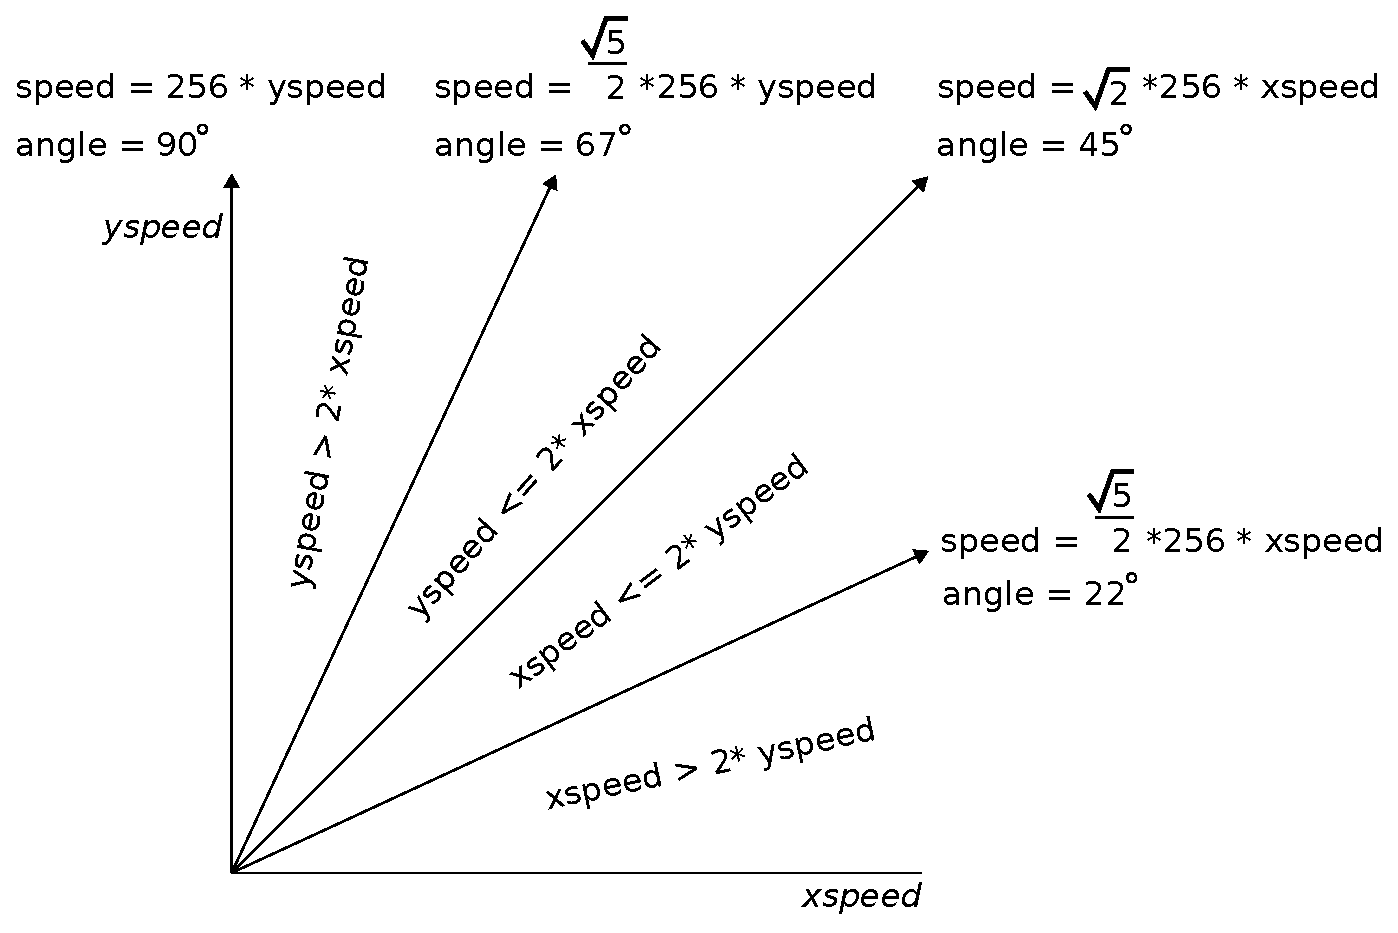
\includegraphics[width=0.8\textwidth]{imgs/drawings/angle.eps}
\label{fig:angles}
\end{figure}
\par
For each of the eight type of slopes (Figure \ref{fig:walltype}) and incoming angle combination, the corresponding bounce is defined using a simple lookup table.\\

\par
Notice that the bounce is not always following the laws of physics. 





\end{document}



